\icode{N23-ME-CA-L3-261019-001}
\nceeID[12]{2023全国甲}{24}
如图，光滑水平桌面上有一轻质弹簧，其一端固定在墙上。用质量为\(m\)的小球压弹簧的另一端，使弹簧的弹性势能为\(E_p\)。释放后，小球在弹簧作用下从静止开始在桌面上运动，与弹簧分离后，从桌面水平飞出。小球与水平地面碰撞后瞬间，其平行于地面的速度分量与碰撞前瞬间相等；垂直于地面的速度分量大小变为碰撞前瞬间的\(\frac{4}{5}\)。小球与地面碰撞后，弹起的最大高度为\(h\)。重力加速度大小为\(g\)，忽略空气阻力。求：
\begin{enumerate}
	\item 小球离开桌面时的速度大小；
	\item 小球第一次落地点距桌面上其飞出点的水平距离。
\end{enumerate}
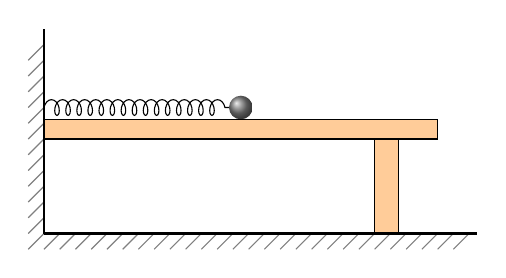
\begin{tikzpicture}
	\draw[decoration={aspect=.6, segment length=4,amplitude=1mm,coil},decorate] (0,0)--(2.4,0);
	\shade[ball color=gray] (2.5,0) circle(.15);
	\draw[fill=orange!40] (0,-.15) rectangle(5,-.4) (4.2,-.4) rectangle(4.5,-1.6);
	\foreach \x in {-.2,0,...,5.3}
		\draw[gray] (\x,-1.8)--++(.2,.2);
	\foreach \y in {-1.6,-1.4,...,.8}
		\draw[gray] (-.2,\y)--++(.2,.2);
	\draw[thick] (0,-1.6)--(5.5,-1.6) (0,-1.6)--(0,1);
\end{tikzpicture}